% Display math whose body is only a picture, with hyperref: a tikzpicture
% in $$ $$, an \includegraphics in \[ \], a numbered equation with a
% \label and an \eqref, and a picture in a theorem. Each case follows a
% paragraph that names it.
\documentclass{article}
\usepackage{amsmath}
\usepackage{amsthm}
\usepackage{graphicx}
\usepackage{tikz}
\usepackage{hyperref}
\newtheorem{theorem}{Theorem}
\begin{document}
Dollars tikzpicture.
$$ \begin{tikzpicture}\draw[->] (0,0) -- (2,0);\end{tikzpicture} $$

Bracket graphics.
\[ 
\includegraphics[alt={hyperref graphics},width=2cm]{test-picture.png} \]

Equation tikzpicture.
\begin{equation}
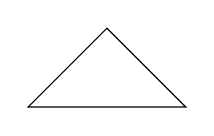
\begin{tikzpicture}\draw (0,0) -- (2,0) -- (1,1) -- cycle;\end{tikzpicture}
\label{eq:triangle}
\end{equation}

\begin{theorem}
Theorem tikzpicture.
\[ 
\begin{tikzpicture}\draw (0,0) rectangle (1,1);\end{tikzpicture} \]
\end{theorem}

Reference to the triangle: \eqref{eq:triangle}.

Ordinary display.
\[ y = 1 \]
\end{document}
